\documentclass[11pt]{article}
\usepackage{enumerate}
\usepackage{fullpage}
\usepackage{fancyhdr}
\usepackage{amsmath, amsfonts, amsthm, amssymb}
\usepackage{graphicx}
\usepackage{wasysym}
\setlength{\parindent}{0pt}
\setlength{\parskip}{5pt plus 1pt}
\pagestyle{empty}

\def\indented#1{\list{}{}\item[]}
\let\indented=\endlist

\newcounter{questionCounter}
\newcounter{partCounter}[questionCounter]
\newenvironment{question}[2][\arabic{questionCounter}]{%
    \setcounter{partCounter}{0}%
    \vspace{.25in} \hrule \vspace{0.5em}%
        \noindent{\bf #2}%
    \vspace{0.8em} \hrule \vspace{.10in}%
    \addtocounter{questionCounter}{1}%
}{}
\renewenvironment{part}[1][\alph{partCounter}]{%
    \addtocounter{partCounter}{1}%
    \vspace{.10in}%
    \begin{indented}%
       {\bf (#1)} %
}{\end{indented}}

%%%%%%%%%%%%%%%%%%%%%%%HEADER%%%%%%%%%%%%%%%%%%%%%%%%%%%%%%
\newcommand{\myname}{Shashank Singh\footnote{sss1@andrew.cmu.edu}
        \footnote{Machine Learning Department \& Department of Statistics}}
\newcommand{\myclass}{10-715 Advanced Introduction to Machine Learning}
\newcommand{\myhwnum}{1}
\newcommand{\duedate}{Thursday, Wednesday October 1, 2014}
%%%%%%%%%%%%%%%%%%%%%%%%%%%%%%%%%%%%%%%%%%%%%%%%%%%%%%%%%%%

%%%%%%%%%%%%%%%%%%%%CONTENT MACROS%%%%%%%%%%%%%%%%%%%%%%%%%
\renewcommand{\qed}{\quad \ensuremath{\blacksquare}}
\newcommand{\inv}{^{-1}}
\newcommand{\bv}{\mathbf{v}}
\newcommand{\bx}{\mathbf{x}}
\newcommand{\by}{\mathbf{y}}
\newcommand{\bff}{\mathbf{f}}
\newcommand{\bzero}{\mathbf{0}}
\newcommand{\bxi}{\boldsymbol{\xi}}
\newcommand{\boldeta}{\boldsymbol{\eta}}
\newcommand{\dist}{\operatorname{dist}}
\newcommand{\area}{\operatorname{area}}
\newcommand{\vspan}{\operatorname{span}}
\newcommand{\Gr}{\operatorname{Gr}} % graph of a function
\renewcommand{\sp}{\operatorname{span}} % span of a set
\newcommand{\sminus}{\backslash}
\newcommand{\E}{\mathbb{E}} % expected value
\newcommand{\F}{\mathcal{F}}
\newcommand{\pr}{\mathbb{P}} % probability
\newcommand{\Var}{\operatorname{Var}} % variance
\newcommand{\N}{\mathbb{N}} % natural numbers
\newcommand{\Z}{\mathbb{Z}} % integers
\newcommand{\Q}{\mathbb{Q}} % rational numbers
\newcommand{\R}{\mathbb{R}} % real numbers
\newcommand{\A}{\mathcal{A}}
\newcommand{\B}{\mathcal{B}}
\newcommand{\C}{\mathcal{C}} % compact functions
\newcommand{\K}{\mathbb{K}} % underlying field of a linear space
\newcommand{\Ran}{\mathcal{R}} % range of a linear operator
\newcommand{\Nul}{\mathcal{N}} % null-space of a linear operator
\renewcommand{\L}{\mathcal{L}} % bounded linear functions
\newcommand{\pow}[1]{\mathcal{P}\left(#1\right)} % power set of #1
\newcommand{\e}{\varepsilon} % \varepsilon
\newcommand{\wto}{\rightharpoonup} % weak convergence
\newcommand{\wsto}{\stackrel{*}{\rightharpoonup}} % weak-* convergence
\renewcommand{\P}{\mathbb{P}}   % probability
\newcommand{\ind}{\perp\!\!\!\perp} % independent
%%%%%%%%%%%%%%%%%%%%%%%%%%%%%%%%%%%%%%%%%%%%%%%%%%%%%%%%%%%

\begin{document}
\thispagestyle{plain}

{\Large Homework \myhwnum, Problems 1 and 2} \\
Name: \myname \\
\myclass \\
Due: \duedate \\
Collaborators: Bryan Hooi

\section{Regression (Samy)}
\subsection{Multi-Task Regression}
\begin{enumerate}
\item Since
$\|Y - \Theta X\|_F^2
    = \sum_{\ell = 1}^k \|\vec y_\ell - \vec \theta_\ell^T X\|_F^2$ and no
element of $\Theta$ is involved in more than one task, the total cost is
minimized precisely by minimizing the cost on each individual task.
\item
\begin{enumerate}
\item Since $\|\Theta\|_F^2 = \sum_{\ell = 1}^k \|\vec\theta_\ell\|_F^2$, the
tasks are still independent. Also, as a norm, $\|\cdot\|_F^2$ is convex. These
properties make $J$ easy to minimize as $k$ convex problems in $d$ dimensions.
\item $\C$ couples the tasks, but, as a sum of norms, $\C$ is convex, so
$\hat \Theta$ can still be found efficiently. Similar to the group lasso, $\C$
encourages columns of $\hat \Theta$ to be zero, and hence identifies components
of $X$ that are most informative.
\item The tasks are neither independent nor convex. However, by encouraging a
low-rank $\hat\Theta$, $\C$ may identify certain tasks or components of $X$
that are most informative, and hence allow for a sparse representation after a
change of coordinates.
\end{enumerate}
\end{enumerate}
\subsection{Shrinkage in Ridge Regression}
\begin{enumerate}
\item Since the objective function is smooth and convex,
\[0
    = \nabla_{\hat\beta} \|X\hat\beta - y\|_2^2 + \lambda\|\hat\beta\|_2^2
    = 2(X\beta - y)^TX + 2\lambda\hat\beta^T.
\]
Hence, since $U$ and $V$ are orthogonal and $\Sigma$ is diagonal,
\begin{align*}
y^TX
    = (X\hat\beta)^TX + \lambda\hat\beta
 &  = (U\Sigma V^T\hat\beta)^TU\Sigma V^T + \lambda\hat\beta^T  \\
 &  = \hat\beta^T V \Sigma U^T U\Sigma V^T + \lambda\hat\beta^T   \\
 &  = \hat\beta^T V \Sigma^2 V^T + \lambda\hat\beta^T
    = \hat\beta^T \Sigma^2 + \lambda\hat\beta^T
    = (\Sigma^2 + \lambda I) \hat\beta^T.
\end{align*}
Thus, noting that both $\lambda$ and the singular values of $X$ are
nonnegative (so $\Sigma^2 + \lambda I$ is invertible),
\[x_*^T\hat\beta
    = \hat\beta^Tx_*
    = (\Sigma^2 + \lambda I)\inv y^T U \Sigma V^T V z_*
    = (\Sigma^2 + \lambda I)\inv y^T U \Sigma z_*
    = \sum_{i = 1}^d \frac{z_{*i}\sigma_i}{\sigma_i^2 + \lambda}u_i^Ty. \qed
\]
\item Without the $L_2$ penalty (i.e., when $\lambda = 0$),
$x_*^T\hat\beta = \sum_{i = 1}^d \frac{z_{*i}}{\sigma_i}u_i^Ty$, and so the
prediction is highly sensitive to small singular values of $X$ (e.g., when
covariates are correlated).
\end{enumerate}
\subsection{Local/Weighted Linear Regression}
\begin{enumerate}
\item Since the objective function is smooth and convex,
\[0
    = \nabla_{\hat\beta} \sum_{i = 1}^n w_i(x)(y_i - \hat\beta x_i)^2
    = 2\sum_{i = 1}^n w_i(x)(\hat\beta x_i - y_i) x_i
    = 2(X\hat\beta - y)^TWX.
\]
Solving for $\hat\beta$ gives $\hat\beta = (X^TWX)\inv X^TWy$, so
$\hat f(x) = x^T\hat\beta = x^T(X^TWX)\inv X^TWy$. \qed
\item Since the objective function is smooth and convex,
\[0
    = \frac{d}{d\hat\theta} \sum_{i = 1}^n w_i(x)(\hat\theta - y_i)^2
    = 2\sum_{i = 1}^n w_i(x)(\hat\theta - y_i).
\]
Solving for $\hat\theta$ gives
$\hat f(x)
    = \hat\theta
    = \frac{\sum_{i = 1}^n w_i(x)y_i}{\sum_{i = 1}^n w_i(x)}$,
which is the Nadaraya-Watson Estimator. Since the
$w_i(x)/\sum_{i = 1}^n w_i(x)$ coefficients are non-negative and add to $1$,
$\hat f(x)$ is a convex combination of $y_i$'s, and so
$\hat f(x) \in (\min_i y_i, \max_i y_i)$. \qed
\end{enumerate}
\subsection{Least Norm Solution}
\begin{enumerate}
\item Let \fbox{$\hat\beta := X^T(XX^T)\inv y$} (noting that, since $X$ has
full rank, $XX^T$ is invertible). Then, $X\hat\beta = XX^T(XX^T)\inv y = y$.
Also, for all $\beta$ with $y = X\beta$,
\[(\beta - \hat\beta)^T\hat\beta
    = (\beta - \hat\beta)^T X^T(XX^T)\inv y
    = (X\beta - X\hat\beta) (XX^T)\inv y
\]
By the Pythagorean Theorem,
$\|\beta\|_2^2
    = \|\beta - \hat\beta\|_2^2 + \|\hat\beta\|_2^2
    \geq \|\beta\|_2^2$,
so $\hat\beta$ is the least norm solution.
\item Note that, since $XX^+$ is symmetric and $XX^+X = X$,
\[(X\beta)^TX
    = (XX^+y)^TX
    = y^TXX^+X
    = y^TX.
\]
Since $\|X\beta - y\|_2^2$ is smooth and convex in $\beta$, to see that
$\hat\beta$ minimizes $\|X\beta - y\|_2^2$, is suffices to observe that
\[\nabla_\beta \|X\beta - y\|_2^2 \big|_{\beta = \hat\beta}
    = 2(X\hat\beta - y)^TX
    = 2(X\beta)^TX - 2y^TX
    = 0.
\]
Now suppose $\beta \in \R^d$ also minimizes $\|y - X\beta\|_2^2$. Then, both
$X\beta$ and $X\hat\beta$ are the projection of $y$ onto the column space of
$X$, so that $X\beta = X\hat\beta$, and hence $\beta - \hat\beta$ is in the
null space of $X$. Since $\hat\beta = X^+y$ is in the column space of $X^+$,
which is the column space of $X^T$, $\hat\beta$ is orthogonal to
$\beta - \hat\beta$. Thus, by the Pythagorean Theorem,
\[\|\beta\|_2^2
    = \|\beta - \hat\beta + \hat\beta\|_2^2
    = \|\beta - \hat\beta\|_2^2 + \|\hat\beta\|_2^2
    \geq \|\hat\beta\|_2^2.
\]
Hence $\hat\beta$ is also the least-norm minimizer of $\|y - X\beta\|_2$. \qed
\end{enumerate}

\section{P\'olya Discriminant Analysis (Samy)}
\subsection{Model}
\begin{enumerate}
\item Note that, whenever $i \neq j$,
$(x_i,y_i) \ind (x_j,y_j) | \theta,\alpha_1,\dots,\alpha_K$, and that
$x_i \ind \theta, \alpha_j | y_i$. Hence,
\begin{align*}
L(\theta,\alpha_1,\dots,\alpha_K)
 &  = p(x_1,\dots,x_n,y_1,\dots,y_n | \theta,\alpha_1,\dots,\alpha_K)   \\
 &  = \prod_{i = 1}^n p(x_i,y_i | \theta,\alpha_1,\dots,\alpha_K)       \\
 &  = \prod_{i = 1}^n p(x_i | y_i,\theta,\alpha_1,\dots,\alpha_K)
                            p(y_i | \theta,\alpha_1,\dots,\alpha_K)
    = \prod_{i = 1}^n p(x_i | \alpha_{y_i}) p(y_i | \theta).
\end{align*}
by definition of condition probability. Since the Dirichlet distribution is the
conjugate prior to the multinomial distribution, given $x_i$ and
$\alpha_{y_i}$, $p \sim$ Dir$(\alpha_{y_i} + x_i)$. Hence, using the definition
of conditional probability and then plugging in the appropriate probability
density functions and simplifying,
\[p(x_i | \alpha_{y_i})
    = \frac{p(x_i | p, \alpha_{y_i})p(p | \alpha_{y_i})}
            {p(p | x_i,\alpha_{y_i})}
    = \frac{\Gamma \left( \sum_{j = 1}^V \alpha_{y_i,j} + x_{i,j} \right)}
           {\Gamma \left( \sum_{j = 1}^V \alpha_{y_i,j} \right)}
        \prod_{j = 1}^V \frac{\Gamma(\alpha_{y_i,j})}
                             {\Gamma(\alpha_{y_i,j} + x_{i,j})}
\]
Thus,
\begin{align}
\notag
\ell(\theta,\alpha_1,\dots,\alpha_K)
 &  = \log L(\theta,\alpha_1,\dots,\alpha_K)    \\
\notag
 &  = \sum_{i = 1}^n \log \theta_{y_i}
        + \log \Gamma \left( \sum_{j = 1}^V \alpha_{y_i,j} + x_{i,j} \right)
        - \log \Gamma \left( \sum_{j = 1}^V \alpha_{y_i,j} \right)  \\
 &  \quad\quad + \sum_{j = 1}^V
                   \log \Gamma(\alpha_{y_i,j})
                    - \log \Gamma(\alpha_{y_i,j} + x_{i,j}).
\end{align}

\item For $i \in \{1,\dots,K\}$, let $c_i$ denote the number of documents in
category $i$. Then, the component of $\ell$ depending on $\theta$ is
\[\ell_\theta(\theta)
    = \sum_{i = 1}^K c_i \log \theta_i
    = \left( \sum_{i = 1}^{K - 1} c_i \log \theta_i \right)
        + c_K \log \left( 1 - \sum_{i = 1}^{K - 1} \theta_i \right),
\]
where the last step follows from $\theta \in \Delta^{K - 1}$. Since
$\ell_\theta$ is smooth and convex in $\theta$, if $\hat\theta$ is the maximum
likelihood estimator of $\theta$, for each $i \in \{1,\dots,K - 1\}$,
\[0
    = \nabla_{\hat\theta_i} \ell_\theta(\hat\theta)
    = \frac{c_i}{\theta_i} - \frac{c_K}{1 - \sum_{i = j}^{K - 1} \theta_j}
    = \frac{c_i}{\theta_i} - \frac{c_K}{\theta_K},
\]
so that $\theta_i = c_i\theta_K/c_K$. Plugging this into
$\sum_{i = 1}^K \theta_i = 1$ and solving for $\theta_K$ gives
$\theta_K = c_K/n$, and it follows that each \fbox{$\theta_i = c_i/n$.}
\item For each $r \in [n], s,t \in [V]$ with ($s \neq t$), most terms in $\ell$
vanish upon differentiation by $\alpha_{i,j}$:
\[\frac{d\ell(\theta,\alpha_1,\dots,\alpha_K)}{d\alpha_r^{(s)}}
    = \sum_{i : y_i = r}^n
        \psi\left( \sum_{j = 1}^V \alpha_r^{(j)} + x_i^{(j)} \right)
        - \psi\left( \sum_{j = 1}^V \alpha_r^{(j)} \right)
        + \psi\left( \alpha_r^{(s)} \right)
        - \psi\left( \alpha_r^{(s)} + x_i^{(s)} \right)
\]
and so
\[\frac{d^2\ell(\theta,\alpha_1,\dots,\alpha_K)}
       {\left( d\alpha_r^{(s)} \right)^2}
    = \sum_{i : y_i = r}^n
        \psi^{(1)}\left( \sum_{j = 1}^V \alpha_r^{(j)} + x_i^{(j)} \right)
        - \psi^{(1)}\left( \sum_{j = 1}^V \alpha_r^{(j)} \right)
        + \psi^{(1)}\left( \alpha_r^{(s)} \right)
        - \psi^{(1)}\left( \alpha_r^{(s)} + x_i^{(s)} \right)
\]
and
\[\frac{d^2\ell(\theta,\alpha_1,\dots,\alpha_K)}
       {d\alpha_r^{(s)}d\alpha_r^{(t)}}
    = \sum_{i : y_i = r}^n
        \psi^{(1)}\left( \sum_{j = 1}^V \alpha_r^{(j)} + x_i^{(j)} \right)
        - \psi^{(1)}\left( \sum_{j = 1}^V \alpha_r^{(j)} \right)
\]
where $\psi$ denotes the digamma function (derivative of $\log\circ\Gamma$) and
$\psi^{(1)}$ denotes its derivative. In particular, if $\ell_{\alpha_r}$
denotes the component of $\ell$ that depends on $\alpha_r$, then the Hessian of
$\ell_{\alpha_r}$ is
$H_{\alpha_r} \ell(\theta,\alpha_1,\dots,\alpha_K)
    = D_{\alpha_r} + c_{\alpha_r}1_V1_V^T$, where
\[D_{\alpha_r} = \sum_{i : y_i = r}
        \operatorname{diag}\left(\psi(\alpha_r^{(1)})
                                    - \psi(\alpha_r^{(1)} + x_i^{(1)}),
            \dots,
            \psi(\alpha_r^{(V)}) - \psi(\alpha_r^{(V)} + x_i^{(V)})\right),
\]
\[c_{\alpha_r}
    = \sum_{i : y_i = r}^n
        \psi^{(1)}\left( \sum_{j = 1}^V \alpha_r^{(j)} + x_i^{(j)} \right)
        - \psi^{(1)}\left( \sum_{j = 1}^V \alpha_r^{(j)} \right),
\]
and $1_V \in \R^V$ denotes the $V$ dimensional column vector of all ones. Since
$D_{\alpha_r}$ is diagonal, $D_{\alpha_r}$ can be represented and inverted in
$\tilde O(V)$ time and space. Thus, we can use the Sherman-Morrison inversion
formula:
\[\left[H\ell_{\alpha_r}(\alpha_r) \right]\inv
    = \left( D_{\alpha_r} + c_{\alpha_r}1_V1_V^T \right)\inv
    = D_{\alpha_r}\inv
        - \frac{D_{\alpha_r}\inv c_{\alpha_r}1_V1_V^TD_{\alpha_r}\inv}
               {1 + c_{\alpha_r}1_V^TD_{\alpha_r}\inv1_V}.
\]
Hence, since the Newton update is
\[\hat\alpha_r \to
    \hat\alpha_r -
    \left[H\ell_{\alpha_r}(\hat\alpha_r) \right]\inv
    \nabla\ell_{\alpha_r}(\hat\alpha_r)
    = \hat\alpha_r -
    \left( D_{\hat\alpha_r}\inv
    - \frac{D_{\hat\alpha_r}\inv c_{\hat\alpha_r}1_V1_V^TD_{\hat\alpha_r}\inv}
           {1 + c_{\hat\alpha_r}1_V^TD_{\hat\alpha_r}\inv1_V} \right)
    \nabla\ell_{\alpha_r}(\hat\alpha_r).
\]
Note that, if the multiplication by $\nabla\ell_{\alpha_r}(\hat\alpha_r)$ is
distributed over the subtraction, as long as $D$ is stored as a $V$ dimensional
vector and all multiplications are performed from right to left, the above
update requires only $8$ vector arithmetic operations on $V$-dimensional
vectors, while storing at most $2$ $V$-dimensional vectors at a time. Hence,
the update can be performed in $\tilde O(V)$ time and space. \qed
\item I didn't have time to finish this. \frownie
\item I didn't have time to finish this. \frownie
\end{enumerate}
\subsection{Experiment}
I didn't have time to get this working. \frownie

\newpage
\setcounter{footnote}{0}
{\Large Homework \myhwnum, Problems 3 and 4} \\
Name: \myname \\
\myclass \\
Due: \duedate

\section{Duality (Veeru)}
\subsection{Weak Duality}
\begin{enumerate}
\item
$L(x,\lambda,u) = f(x) + \lambda h_1(x) + u h_2(x)$.
\item
$\displaystyle g(\lambda,u)
    = \inf_{x \in \R^d} L(x,\lambda,u)
    = f(x) + \lambda h_1(x) + u h_2(x)$.
\item For any primal feasible $x$ and dual feasible $\lambda$ and $u$,
$h_1(x) \leq 0$, $h_2(x) = 0$, and $\lambda \geq 0$. Thus,
\[g(\lambda^*,u^*)
    \leq L(x^*, \lambda^*, u^*)
    = f(x^*) + \lambda h_1(x^*) + u h_2(x^*)
    \leq f(x^*). \qed
\]
\end{enumerate}

\subsection{Optimal Coding}
\begin{enumerate}
\item Since any exponential function and any sum of convex functions are
necessarily convex, the first constraint is convex. Since the second constraint
is trivially convex and the intersection of two convex sets is convex, the
feasible region is convex. \qed

\item Note that the objective is non-increasing in each component of $x$, and
that, by the first constraint, any feasible $x$ has only strictly positive
components. Thus, for all $x \in \R_+^n$ $x_i$, unless equality holds in the
first constraint, we can reduce the objective function by replacing $x_i$ by
$x_i - \e$ for some $\e > 0$ (since the first constraint is continuous in $x$).
Hence, $x$ is optimal only if the first constraint is tight. \qed

\item By stationarity, $\exists u \in \R$ such that, for each
$i \in \{1,\dots,n\}$,
\[0
    = \frac{d}{dx_i} \sum_{i = 1}^n p_i x_i
                        + u \left( \sum_{i = 1}^n 2^{-x_i} - 1\right)
    = p_i - u \ln(2) 2^{-x_i}.
\]
Hence, $2^{-x_i} = \frac{p_i}{u \ln(2)}$. Since the sum of $p_i$'s is $1$,
\[1
    = \sum_{i = 1}^n 2^{-x_i}
    = \sum_{i = 1}^n \frac{p_i}{u \ln(2)} = \frac{1}{u \ln(2)},
\]
and so $u = 1/\ln(2)$. Thus, \fbox{$x_i = -\log_2 p_i$.}
\end{enumerate}

\section{SVM and Perceptron (Veeru)}
\subsection{Finding support vectors from dual variables}
The KKT conditions give that, for some
$\lambda_1,\dots,\lambda_n,\mu_1,\dots,\mu_n \leq 0$, $u \in \R$, for each
$i \in [n]$, by Stationarity,
\begin{align*}
0
 &  = \frac{1}{2} \sum_{j \neq i} \alpha_jy_iy_j \langle x_i, x_j \rangle
        + \alpha_iy_i^2 \|x_i\|^2 - 1
        + uy_i + \lambda_i - \mu_i \\
 &  = \frac{1}{2} y_i \langle x_i, \sum_{j \neq i} \alpha_j y_j x_j \rangle
        + \alpha_i \|x_i\|^2 - 1
        + uy_i + \lambda_i - \mu_i \\
 &  = \frac{1}{2} y_i \langle x_i, w - x_i \rangle
        + \alpha_i \|x_i\|^2 - 1
        + uy_i + \lambda_i - \mu_i  \\
 &  = \frac{1}{2} y_i \langle x_i, w \rangle
        + (\alpha_i - y_i/2) \|x_i\|^2 - 1
        + uy_i + \lambda_i - \mu_i  \\
 &  = \frac{1}{2} y_i (f(x_i) - b)
        + (\alpha_i - y_i/2) \|x_i\|^2 - 1
        + uy_i + \lambda_i - \mu_i,
\end{align*}
since $y_if(x_i) = y_i \langle w, x_i \rangle + y_ib$. By complementary
slackness, if $\alpha_i < C$, then $\mu_i = 0$, and so
\[y_if(x_i)
    = b + (y_i - 2\alpha_i)\|x_i\|^2 + 2 - uy_i - \lambda_i
    \geq b + (y_i - 2\alpha_i)\|x_i\|^2 + 2 - uy_i,
\]
since $\lambda_i \leq 0$. Similarly, if $\alpha_i > 0$, then $\lambda_i = 0$,
so, since $\mu_i \leq 0$,
\[y_if(x_i)
    = b + (y_i - 2\alpha_i)\|x_i\|^2 + 2 - uy_i + \mu_i
    \leq b + (y_i - 2\alpha_i)\|x_i\|^2 + 2 - uy_i.
\]
Hence, it suffices to show $b + (y_i - 2\alpha_i)\|x_i\|^2 - uy_i = -1$. Didn't
have time to go further. \frownie
\subsection{Using libsvm}
See Figures \ref{fig:4.2.1}, \ref{fig:4.2.2}, and \ref{fig:4.2.3} below. Code
is attached on the last page.
\begin{figure}[h!]
\begin{center}
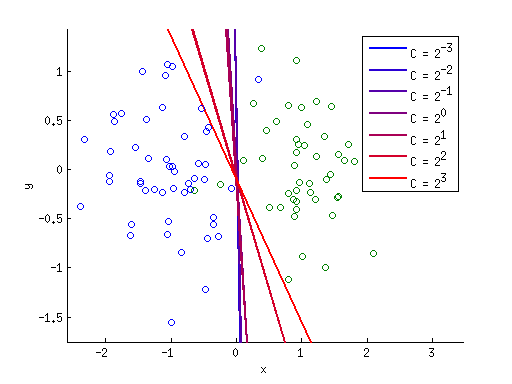
\includegraphics[width=0.68\textwidth]{4_2_1}
\end{center}
\vspace{-9mm}
\caption{Decision boundaries of SVM for various values of $C$, over the
training data.}
\label{fig:4.2.1}
\end{figure}
\begin{figure}[h!]
\begin{center}
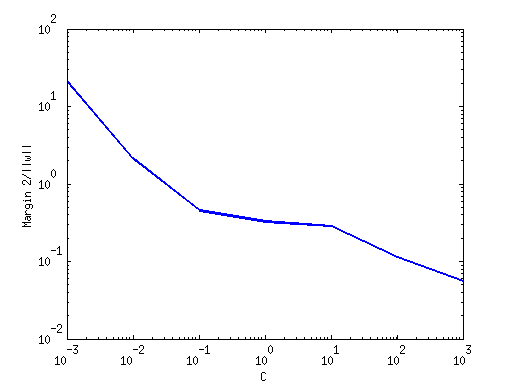
\includegraphics[width=0.68\textwidth]{4_2_2}
\end{center}
\vspace{-9mm}
\caption{Log-log plot of width of SVM margin for various values of $C$.}
\label{fig:4.2.2}
\end{figure}
\begin{figure}[h!]
\begin{center}
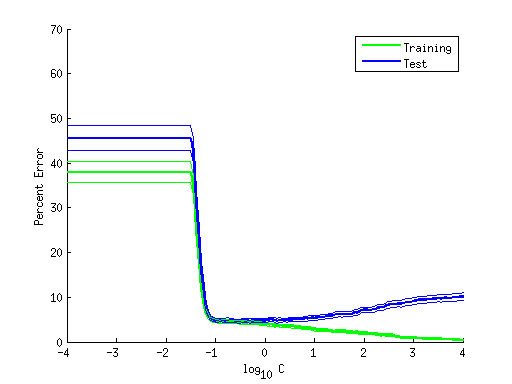
\includegraphics[width=0.65\textwidth]{4_2_3}
\end{center}
\vspace{-9mm}
\caption{Semilog plot of test error and training error for various values of
$C$, averaged over $50$ trials, with standard error bands.}
\label{fig:4.2.3}
\end{figure}

\subsection{Mistake bound for Perceptron}
\begin{enumerate}
\item Clearly, for $k = 0$,
$\langle w_0, w_* \rangle = \langle 0, w_* \rangle = 0 = k\delta$. If
$\langle w_k, w_* \rangle \geq k\delta$ for some $k \geq 0$, then,
\[\langle w_{k + 1}, w_* \rangle
    = \langle w_k + y_{i(k + 1)}x_{i(k + 1)}, w_* \rangle
    = \langle w_k, w_* \rangle + y_{i(k + 1)}\langle x_{i(k + 1)}, w_* \rangle
    \geq k\delta + \delta
    = (k + 1)\delta. \qed
\]
\item Clearly, for $k = 0$, $\|w_k\|^2 = 0 = kM^2$. If $\|w_k\|^2 \leq kM^2$
for some $k \geq 0$, then
\begin{align*}
\|w_{k + 1}\|^2
    = \|w_k + y_{i(k + 1)}x_{i(k + 1)}\|^2
 &  = \|w_k\|^2
        + 2\langle w_k, y_{i(k + 1)}x_{i(k + 1)} \rangle
        + |y_{i(k + 1)}|\|x_{i(k + 1)}\|^2  \\
 &  = kM^2 + 2y_{i(k + 1)}\langle w_k, x_{i(k + 1)} \rangle + M^2
    \leq (k + 1)M^2,
\end{align*}
since $w_k$ fails on $(y_{i(k + 1)},x_{i(k + 1)})$, so that
$2y_{i(k + 1)}\langle w_k, x_{i(k + 1)} \rangle \leq 0$. \qed
\item For all iterations $k$ such that the algorithm still makes mistakes, by
Cauchy-Schwarz,
\[(k\delta)^2
    \leq \langle w_k, w_* \rangle^2
    \leq \|w_k\|^2\|w_*\|^2
    = \|w_k\|^2
    \leq kM^2.
\]
Hence, $k_* \leq M^2/\delta^2$. \qed
\end{enumerate}

\end{document}
